%%%% Header %%%%%%%%%%%%%%%%%%%%%%%%%%%%%%%%%%%%%%%%%%%%%%%%%%%%%%%%%%%%%%%%%%%

\documentclass[a4paper]{scrartcl}

%%%% Packages %%%%%%%%%%%%%%%%%%%%%%%%%%%%%%%%%%%%%%%%%%%%%%%%%%%%%%%%%%%%%%%%%

% font/encoding
\usepackage[utf8]{inputenc}          % .tex-file text encoding
\usepackage[T1]{fontenc}             % vector fonts and hiQual special chars in output
\usepackage{libertine}               % libertine font family
\usepackage[libertine]{newtxmath}    % libertine mathematics
\usepackage[scaled=0.9]{inconsolata} % monospace font

% localization
\usepackage[english]{babel}         % document language/localization
\usepackage[babel = true]{csquotes} % global quotation style
                                    % dependent on language
\usepackage[htt]{hyphenat}          % hyphenation rules

% maths
\usepackage{mathrsfs} % maths script fonts
\usepackage{amssymb}  % maths symbols
\usepackage{amsmath}  % various maths features
\usepackage{units}    % unit handling and nice fractions

% page layout
\usepackage{chngpage}          % allows for temporary adjustment of side margins
\usepackage{lscape}            % use a page in landscape orientation
\usepackage[a4paper]{geometry} % ability to change margins

% lists
\usepackage{paralist} % compact versions of standard lists environments

% colours
\usepackage[usenames, table]{xcolor} % colour support

% figures
\usepackage{graphicx}   % include external images
\usepackage{tikz}       % generate vector graphics in latex
\usepackage{wrapfig}    % environment where text will flow around images
\usepackage[format          = plain, % configure captions
            indention       = .3cm,
            margin          = 20pt,
            font            = small,
            labelfont       = bf,
            justification   = raggedright,
            singlelinecheck = on]{caption}
\usepackage{subcaption} % captions for subfigures

% tables
\usepackage{dcolumn}        % column alignment at decimal point
\usepackage{threeparttable} % new table environment for better annotations
\usepackage{booktabs}       % nice table rules

% typography
\usepackage{setspace} % set space between lines

% bibliography
\usepackage[style = authoryear-ibid, % bibliography using biblatex
            backend = biber,
            bibencoding = utf8,
            doi = false,
            isbn = false]{biblatex}

% verbatim
\usepackage{listings} % source code environment

% symbols
\usepackage{MnSymbol} % various symbols (used to mark linebreaks in listing)

%%%% Paths %%%%%%%%%%%%%%%%%%%%%%%%%%%%%%%%%%%%%%%%%%%%%%%%%%%%%%%%%%%%%%%%%%%%

% bibliography file
\bibliography{/home/jon/lucile/share/hive/sci/refs/refs.bib}

%%%% Listings %%%%%%%%%%%%%%%%%%%%%%%%%%%%%%%%%%%%%%%%%%%%%%%%%%%%%%%%%%%%%%%%%

% listings caption style
\renewcommand{\lstlistingname}{Script} % caption name
\DeclareCaptionFormat{listing}{\raisedrule[0.3em]{0.5pt}~\mbox{#1#2#3}~\raisedrule[0.3em]{0.5pt}}
\captionsetup[lstlisting]{format=listing,
                          singlelinecheck=false,
                          margin=0pt,
                          font={sf},
                          labelsep=space,
                          labelfont=bf}

% help package "listings" to represent german special chars
\lstset{literate=%
{Ö}{{\"O}}1
{Ä}{{\"A}}1
{Ü}{{\"U}}1
{ß}{{\ss}}1
{ü}{{\"u}}1
{ä}{{\"a}}1
{ö}{{\"o}}1
}

\lstset{
language = R,
% sets automatic line breaking
breaklines = true,
% where to put the line-numbers; possible values are (none, left, right)
numbers = left,
% how far the line-numbers are from the code
numbersep = 10pt,
% the style that is used for the line-numbers
numberstyle = \footnotesize,
% number lines 5, 10, 15...
stepnumber=5,firstnumber=1,
% font and size for code
basicstyle = \singlespacing\ttfamily\small,
% mark linebreaks
prebreak = \raisebox{0ex}[0ex][0ex]{\ensuremath{\rhookswarrow}},
postbreak=\raisebox{0ex}[0ex][0ex]{\ensuremath{\rcurvearrowse\space}},
% highlighting
commentstyle=\color{blue},
keywordstyle=\ttfamily\small,
stringstyle=\color{brown},
frame=bottomline,
}

%%%% Hyphenation %%%%%%%%%%%%%%%%%%%%%%%%%%%%%%%%%%%%%%%%%%%%%%%%%%%%%%%%%%%%%%

% global hyphenation rules
\hyphenation{}

%%%% General layout %%%%%%%%%%%%%%%%%%%%%%%%%%%%%%%%%%%%%%%%%%%%%%%%%%%%%%%%%%%

% avoid orphans and widows
\widowpenalty = 10000
\clubpenalty = 10000

% don't break footnotes
\interfootnotelinepenalty = 10000

% don't hyphenate across pages
\brokenpenalty10000\relax

% roman page numbers for appendix
\let\origappendix\appendix % save the existing appendix command
\renewcommand\appendix{\clearpage\pagenumbering{roman}\origappendix}

% make section heading smaller
\addtokomafont{sectioning}{\normalsize}

%%%% Abstract %%%%%%%%%%%%%%%%%%%%%%%%%%%%%%%%%%%%%%%%%%%%%%%%%%%%%%%%%%%%%%%%%

% better abstract environment

\newenvironment{abstract2}{
  \begin{center}
      \begin{minipage}{0.9\linewidth}\small
      \textsc{Abstract.}}{\\
      \end{minipage}
  \end{center}
}

%%%% Tables %%%%%%%%%%%%%%%%%%%%%%%%%%%%%%%%%%%%%%%%%%%%%%%%%%%%%%%%%%%%%%%%%%%

% global table format
\newcommand{\tabformat}{\small\centering}
% fontsize of table footnote
\newcommand{\tabfontsizefoot}{\footnotesize}
% dcolumn column type
\newcolumntype{d}{D{,}{,}}
% centering with fixed column size in tables
\newcolumntype{Q}[1]{>{\centering\arraybackslash}p{#1}}
% raggedright in tables
\newcolumntype{P}[1]{>{\raggedright\hspace{0pt}\arraybackslash}p{#1}}

%%%% Maths %%%%%%%%%%%%%%%%%%%%%%%%%%%%%%%%%%%%%%%%%%%%%%%%%%%%%%%%%%%%%%%%%%%%

% phantom relation signs for alignment
\newcommand\relphantom[1]{\mathrel{\phantom{#1}}}

%%%% Hyphenation %%%%%%%%%%%%%%%%%%%%%%%%%%%%%%%%%%%%%%%%%%%%%%%%%%%%%%%%%%%%%%

% global hyphenation rules
\hyphenation{de-mo-gra-phy po-pu-la-tion dy-na-mics epi-demi-olo-gists im-ple-men-ta-tions}

%%%% Rules %%%%%%%%%%%%%%%%%%%%%%%%%%%%%%%%%%%%%%%%%%%%%%%%%%%%%%%%%%%%%%%%%%%%

% line filling rule
\newcommand{\raisedrule}[2][0em]{\leavevmode\leaders\hbox{\rule[#1]{1pt}{#2}}\hfill\kern0pt}


%%%% Meta data %%%%%%%%%%%%%%%%%%%%%%%%%%%%%%%%%%%%%%%%%%%%%%%%%%%%%%%%%%%%%%%%

\usepackage[pdfauthor={Jonas Schöley, Frans Willekens},
            pdftitle={Visualizing Compositional Data on the Lexis Surface},
            pdfsubject={Visualization},
            pdfkeywords={visualization, colour, compositional data, Lexis surface},
            pdfproducer=Latex,
            pdfcreator=pdflatex]{hyperref}

\title{Visualizing Compositional Data\\on the Lexis Surface\footnote{PAA 2015 conference paper. Presented on April 30 in San Diego at the conference session on \emph{Visualizing Demographic Data}.}}
\author{Jonas Schöley\footnote{The authors work has been funded by the Max Planck Society. Currently he is based in Warsaw as a student of the European Doctoral School of Demography.} \, and Frans Willekens\footnote{Chief Research Coordinator at the Max Planck Institute for Demographic Research in Rostock.}\\
\texttt{schoeley@demogr.mpg.de $\cdot$ willekens@demogr.mpg.de}}
\date{\today}

%%%% Titlepage %%%%%%%%%%%%%%%%%%%%%%%%%%%%%%%%%%%%%%%%%%%%%%%%%%%%%%%%%%%%%%%%

\begin{document}

\maketitle

%%%% Text %%%%%%%%%%%%%%%%%%%%%%%%%%%%%%%%%%%%%%%%%%%%%%%%%%%%%%%%%%%%%%%%%%%%%

\begin{abstract2}
The analysis of compositional data is a topic inherent to demography. In recent times, due to a growing catalogue of detailed population data, it became feasible to consider populations not only structured by time, age or sex, but by any number of interesting criteria. This \enquote{inflation} of data dimensions produces challenges in visualizing the data. To aid the understanding of age-structured timelines of compositions we seek to extend the Lexis surface plot from 1-dimensional continuous data to multidimensional compositional data. We apply different strategies for visualizing compositional data on the Lexis surface to French death counts given by cause and compare the results for compliance with multiple desired criteria.
\end{abstract2}

% Visualizing demographic data
From the display of population numbers by shading map regions, the graphical representation of population dynamics on a grid of year-age-cohort parallels, and the widely recognized population pyramid to today's heatmaps of mortality surfaces: Demography has always had a close relationship with information visualization.\footnote{One of the first choropleth maps of population densities can be found in \textcite{Dangeville1836}. The year-age-cohort grid is commonly attributed to \textcite{Lexis1875} but for a full account of the inventors of the \enquote{Lexis}-diagram cp.~\textcite{Vandeschrick2001}. Population pyramids were first published in \textcite{Walker1874}. In 1987 \textcite{Vaupel1987} discussed the use of heatmaps in a demographic context.} The visual display helps making sense of the data at hand which in demography, for the most part, are \emph{counts, rates and proportions}. Visualisation methods that are currently used in demography present counts or rates. This paper is about \emph{compositional data}, represented by proportions, i.\,e.~shares of a whole. Examples for this data type are proportions within a population (e.\,g.~age composition, distribution by occupation, region of residence or level of education), proportions of events (e.\,g.~deaths by cause), proportions of durations (e.\,g.~life expectancy by health status), and proportions within a total rate (e.\,g.~death rate by cause of death).

% Rates & counts vs. compositional data
While rates and counts provide a \emph{single value} for each point on the Lexis-surface a \emph{vector of values} is needed in the case of compositional data. Classical solutions for the visualization of population dynamics, such as contour maps or a one-dimensional heatmap of continuous data on the Lexis-surface, do not work for compositional data. On the other hand graphs specifically designed for compositional data like the ternary coordinates (\cite{Aitchison1986}:5\,ff) or the biplot (\cite{Gabriel1971, Aitchison2002}) do not address the basic demographic dimensions period, age and cohort and therefore are unsuited to show corresponding effects in a single display.

% Visualising compositional data
This paper aims to extend the visual repertoire of demography by introducing and discussing different techniques of graphing compositional data on the Lexis surface. Hereby we hope to facilitate the exploratory analysis of compositional data and the communication of research results in graphical form. To demonstrate the techniques we use publicly available data on age-specific death counts by cause of death in France from 1925 to 1999 (\cite{Vallin2014}). Four visualizations are discussed in this paper. The first is the three-variable balance scheme or \emph{ternary balance scheme}.\footnote{Ternary refers to a system with three states.} It is a technique to display three attributes in a single point. Each attribute is mapped to a primary colour and the mixture of three colours shows the composition of attributes in a population. The second visualization is the \emph{qualitative sequential scheme}. In that scheme, a qualitative or categorical variable (e.\,g.~cause of death) is represented by a colour and the quantitative variable (e.\,g.~number of deaths due to that cause) is represented by sequences of lightness steps within each colour. The third visualization, the \emph{age-wise area graph}, is composed of stacked area charts drawn separately for every age group and assembled on a Lexis-like grid. The fourth is a collection of heatmaps portraying different subsets of the data. The resulting visualization is also known as trellis plot, lattice chart or panel chart. \cite{Tufte1990} refers to it as \emph{small multiples}. We use this conventional technique as the state-of-the-art to compare our innovations against. Furthermore we propose a slight refinement to the small multiple graph making it more suitable for the display of compositional data.

% Evaluating visualization techniques 
We assess the quality of the proposed visualizations by discussing various aspects and features of each technique. The different visualizations are compared regarding their statistical/demographical features, their ability to communicate precise values as well as general patterns of the data and the practical issue of space economy. Some evaluation criteria, like the kind of statistic that is actually displayed in the visualization, can be assessed precisely. Other questions, like the ability of the visualization to show patterns in the data, are ultimately a matter of subjective judgements. We back up our personal judgements of these subjective criteria by references to experiments done in graphical perception and by demonstration of the visualizations using real world data.

% Evaluation criteria
The evaluation criteria are defined as follows:
\emph{Sufficiency} is the question whether or not all values of the compositional data (e.\,g.~all individual group shares for each period-age) are displayed in the visualization or if only a subset of the group data (e.\,g.~the share of the largest group for each period-age) is visualized.
\emph{Continuity} describes the preservation of the continuous Lexis grid in the visualization, e.g.\, whether or not the period and age axes constitute a rectangular grid unbroken by whitespace or period-wise/age-wise scales.
The \emph{Category limit} is a precise (if limited by technical reasons) or approximate (if limited by perceptional reasons) count of categories in the compositional data which can be displayed at once.
\emph{Pattern perception} describes the \enquote{visual decoding of physical information} (\cite{Cleveland1994}:223\,f). Within the context of our paper this translates into the ability of a visualization for showing period-, age-, and cohort-effects in the composition of the data along the Lexis surface.
\emph{Table look-up} \enquote{[is the] visual decoding of scale information [\ldots]} (\cite{Cleveland1994}:223\,f). It takes place when attempting to extract the exact numbers from a displayed data point. Some visual primitives (such as xy-position, height, size etc.) -- and therefore some visualizations -- make this task easier than others.
The \emph{Footprint} is often of concern when publishing results. Some visualizations gain their descriptive power from a large footprint.

% Structure of paper
In addition to the introduction and the conclusion the paper consists of 7 sections. In Section 2, we briefly present the Lexis surface, which represents the state-of-the-art of visualization of demographic data grouped by age, period (and cohort). The techniques presented in this paper are extensions of the Lexis surface to the domain of compositional data. Section 3 introduces colour terminology and the concepts of colour composition and colour spaces -- matters which are referred to in the subsequent description of the visualizations, sections 4--7. Prior to the conclusion we compare the proposed visualization techniques with each other and assess the individual features according to our evaluation criteria.

\section*{The Lexis Surface}

\begin{wrapfigure}{o}{0cm}
  \centering
  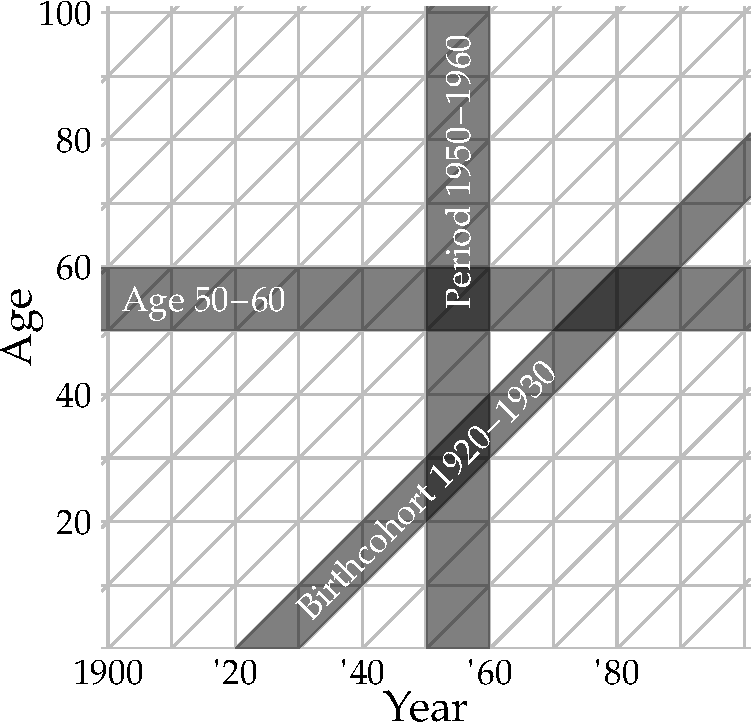
\includegraphics[width = 5cm]{../fig/plot-lexis_exmpl.pdf}
  \caption{The Lexis diagram.}
  \label{fig:lexis_exmpl}
\end{wrapfigure}

% The Lexis diagram
The \emph{Lexis diagram} connects calendar time with age and cohort by the use of a two dimensional diagram with period on the ordinate ($x$) and age on the abscissa ($y$). By interconnecting the three essential time-scales of demography the Lexis diagram serves as an aid in working with population processes and is used to represent events (e.\,g.~birth, death, migration) or occupied states (e.\,g.~single, cohabiting, married, divorced) along the individual life course as well as on the population level. Ages are represented as horizontal parallels, single years as vertical parallels, and each birth cohort is represented by a 45$^\circ$ diagonal. Individuals or populations can be located and tracked on the Lexis diagram as they progresses through time and age (see figure \ref{fig:lexis_exmpl}). The tool is widely used by demographers and epidemiologists to study population and disease dynamics.\footnote{Implementations are available for the statistical software \texttt{R}: The packages \texttt{Epi} (\cite{Carstensen2014}) and \texttt{Biograph} (\cite{Willekens2013b}) both include functions to display data on a time-age-cohort grid.}

% The Lexis surface
The term \emph{Lexis surface} has been introduced by \textcite{Arthur1984} to describe a collection of demographic rates given by discrete time and age. The term now extends to the visualization of population data (counts, rates) across time and age in the form of contour maps or heatmaps (for examples see e.\,g.~\cite{Rau2008, Scherbov2002}). \emph{Contour-maps} indicate regions of equal value for a variable on the time-age plane by a contour line (isoline). \textcite{Vaupel1987} trace the use of these graphs in Demography back to \textcite{Kermack1934} and \textcite{Delaporte1941}. \emph{Heatmaps} express the value of a variable for every point on the time-age plane by the use of colour (e.\,g.~light regions might indicate high values, dark regions in turn low values, see figure \ref{fig:lexis_fx}). \citeauthor{Gambill1985} facilitated the use of these graphs in demography by developing a plotting software running on personal computers: \texttt{LEXIS} (\cite{Gambill1985}) was able to produce \emph{shaded contour maps}, a combination of heatmaps with contour lines, from demographic data. \citetitle{Vaupel1987} showcases the software and the Lexis surface plots across a variety of demographic applications and datasets. Recent refinements to the Lexis surface plot were done by Riffe, who plotted fertility rates structured by period, age \emph{and} cohort resulting in a surface made of triangles instead of rectangles. Riffe also proposed and demonstrated the use of equilateral coordinates to avoid visual distortion along the cohort lines. The programs are written in \texttt{R} and published on Riffes personal webpage (\cite{Riffe2014}).

This paper applies the term \enquote{Lexis surface} to the visual display of compositional population data given on an period-age-grid.

\begin{figure}[htb!]
  \centering
  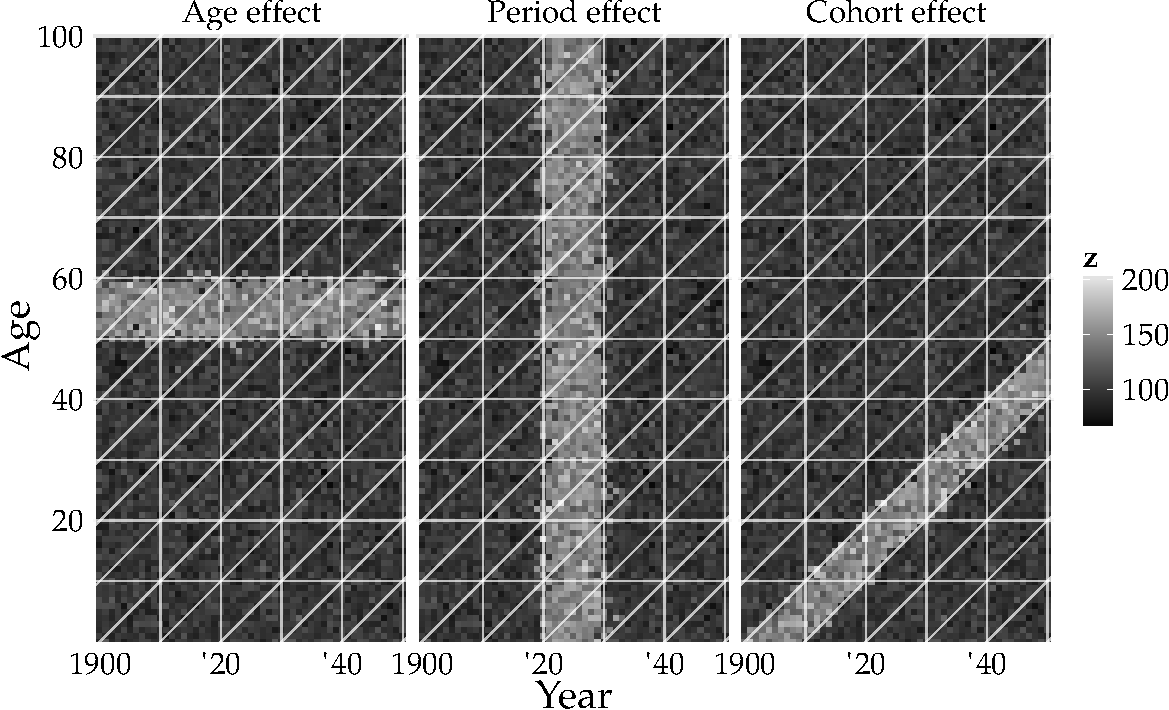
\includegraphics[width = \linewidth]{../fig/plot-lexis_fx.pdf}
  \caption{Heatmap representation of Age-, Period-, and Cohort-effects on the Lexis-surface (simulated data).}
  \label{fig:lexis_fx}
\end{figure}

\section*{About Colour}

% Colour in visualizing compositional data
How to use colour to visualize compositional data? Two of the visualizations presented in this paper -- the ternary-balance-scheme and the qualitative-sequential-scheme -- show possible solutions to that question. The ternary-balance-scheme employs the composite nature of mixed colours to display compositional data. The qualitative-sequential scheme maps different dimensions of colour to different data dimensions. In order to understand these techniques some understanding of colour terminology, colour mixing and colour spaces is needed. We will start off with a familiar setting:

% Primaries and colour mixtures
Children learn how to produce a wide range of colours by mixing blue, red and yellow paints. The resulting colour depends on the ratio between these \emph{primary colours}: Mix yellow with blue to get green, red with blue to get purple and three parts of yellow with one part of red to produce orange. If you want to change the \emph{lightness} of the colour, add either black (darkens) or white (brightens) paints into the mix. Digital printers use the same principle but use a slightly different set of primary colours, namely cyan, yellow and magenta. A colour computer screen uses yet a different set of primaries: its pixels are composed of red, green and blue subpixels. The relative light-output of these subpixels (\emph{luminance}) determines the colour of the pixel. Furthermore, when mixing red, blue and green light sources by equal parts the resulting colour will be white (\emph{additive colour mixing}) whereas mixing yellow, blue and red paints on a canvas will result in a dark brown (\emph{subtractive colour mixing}).

% Complexities of mixing colours
We can see that there is much more to colour mixing than the few rules taught in basic art classes. The choice of primary colours in the end is arbitrary (\cite{Ware2013}:100\,f). There is nothing special about blue, red and yellow. Additionally, when working with coloured light sources you will observe different mixtures compared to working with coloured, reflective surfaces.

% Colour spaces
\emph{Colour spaces} provide a rigorous way to work with colour. They aim to parametrize and quantify it. Some refer to our experiences of how colour is mixed in everyday situations (RGB for light sources, CYMK for printing), others are more abstract. The common ground is the prediction of a colour dependent on a set of input parameters. In case of the RGB colour space -- used to display colours on a television or computer screen -- the input parameters are the amounts of red, green and blue light emitted, commonly encoded with values from 0-255. Here the mixed colour is expressed as a composition of primary colours.

% Perceptional colour dimensions
It is also possible to build a colour space on parameters relating to human colour perception. When asked to describe a colour it would be a remarkable feast for a person to express it in terms of the proportions of primary colours. Instead we tend to say that a colour is bright or dark (\emph{lightness}), tending to blue, red, green or purple (\emph{hue}) and being very neon or more on the grey side (\emph{chroma}, see \cite{Fairchild2005} chapter 4 for colour terminology).

% CIE Lch colour space
The \emph{CIE-Lch} (Lightness, chroma, hue) colour space expresses a colour in terms of these three perceptional parameters. Geometrically it can be thought of as a cylinder filled with different colours. The hue of the colours changes around the circumference, the chroma changes along the radius, with neon colours far out and perfect grey at the centre. The lightness changes along the hight of the cylinder with black at the bottom and white at the top. This colour space is not parametrized in terms of primary colours. Therefore colour mixtures are not to be seen from the parameters. However, choosing multiple points in the CIE-Lch colour space, colour mixtures can be constructed by simple geometric operations (see Appendix A).

% Uniform colour spaces
Apart from an intuitive interpretation of the parameters CIE-Lch has other features making it feasible for use in visualization. Its parameters are not correlated with each other, e.\,g.~changing the lightness will not change the hue or chroma of a colour. Furthermore the function that maps the parameters to the predicted colours is derived from experiments in colour perception. If we specify a range of colours with equal lightness the average observer will perceive the colours as very similar in lightness. On the other hand, the magnitude of perceived differences between two colours will roughly correspond to the magnitude of the quantitative differences in the colour parameters. The usage of such a \emph{uniform} colour space is crucial when translating quantitative data into truthful visual representations (\cite{Ware2013}:105, \cite{Fairchild2005}:185).

\section*{Ternary-Balance-Scheme}

% Colour scheme systematics
Cartographers have a long tradition of using colour for data representation and it comes to no surprise that elaborated systematics on the use of colour emerged in this field. A field-agnostic systematic is proposed by \textcite{Brewer1994a} (see also \cite{Brewer1994}). Starting with the established qualitative-, binary-, sequential- and divergent colour-scales Brewer also addresses combinations of these scales such as the \emph{Three-variable-balance-scheme}.

% Ternary-balance-scheme
The idea is to represent the proportions among three groups with a mixture of three basic colours. The basic colours have different hues, each corresponding to a category of a ternary variable. They are mixed in relations equal to the relations between the three groups in the data. The resulting colour mixture is unique for every possible combination of shares among three groups. The colour-coded ternary diagram can be used as a legend for this type of graph.

% Interpreting the Ternary-balance-scheme
The colours in the ternary-balance-scheme follow two basic principles which facilitate intuitive interpretation of the results:

\begin{compactenum}
  \item The higher the share of a group the more the mixed colour resembles the base colour for that group, and
  \item the more equal the group shares are the more the mixed colour tends to grey.
\end{compactenum}

Using colour mixtures to display multiple data dimensions in a single colour has been proposed several times (e.\,g.~\cite{Trumbo1981}, \cite{Eyton1984}, \cite{Ware1988}). The strength in the ternary-balance-scheme lies within the natural interpretation of its colour-mixtures. It is not necessary to memorize the complete legend to make sense of the data. All the reader has to do is to recall the three basic group colours (like in a categorical colour scale) and the interpretation follows the two simple rules given above. With the use of a ternary diagram as legend we are able to colour-code all possible proportions between three groups in a way reminiscent of the representation of colour spaces in two dimensions.

\begin{figure}[htb!]
\begin{subfigure}[t]{0.65\textwidth}
  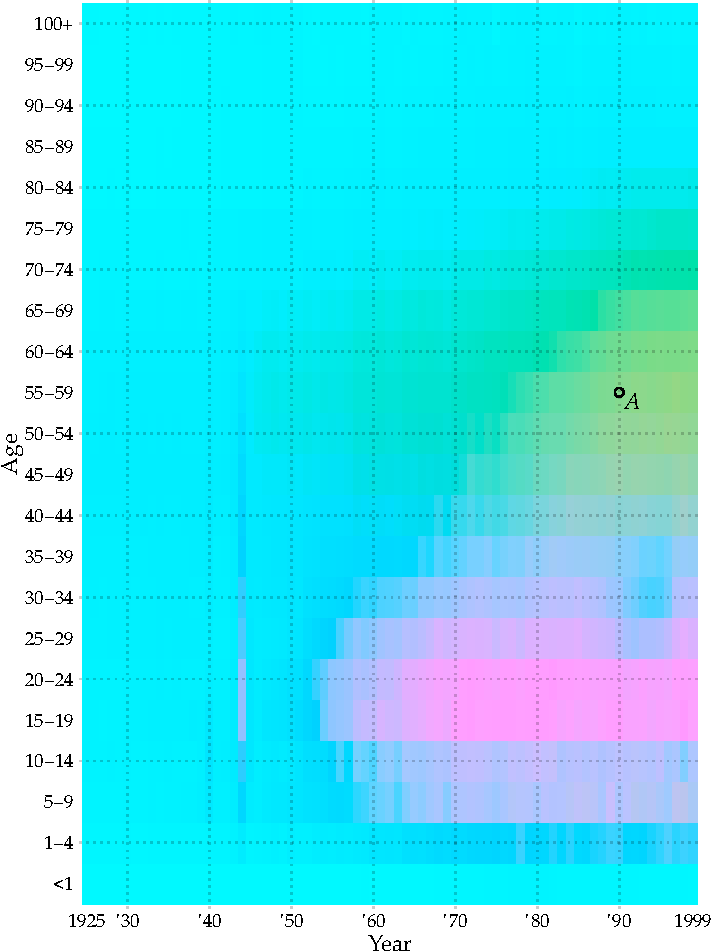
\includegraphics[width = \textwidth]{../fig/plot-tern_balance_no_lgnd.pdf}
  \subcaption{Proportion of people dying from a given cause by time and age (France, total population).}
  \label{fig:tbsplot}
  \end{subfigure}%
  ~
  \begin{subfigure}[t]{0.35\textwidth}
  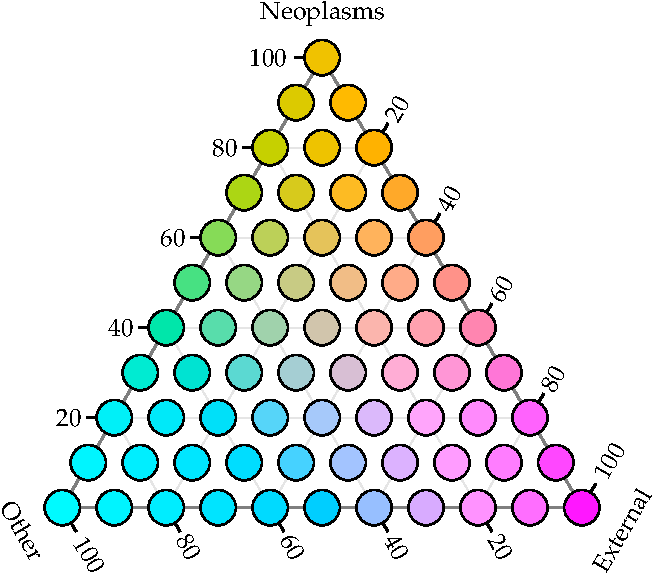
\includegraphics[width = \linewidth]{../fig/plot-tern_balance_lgnd.pdf}
  \subcaption{Legend for Ternary-\hskip0ptbalance-\hskip0ptscheme graph of French cause of death data.}
  \label{fig:tbslegend}
  \end{subfigure}%
  \caption{Ternary-balance-scheme: Proportion of people dying from a given cause by time and age.}
  \label{fig:tbs}
\end{figure}

Figure \ref{fig:tbs} shows the ternary-balance-scheme applied to age-wise French cause-of-death data across the $20^\text{th}$ century. All deaths are divided by cause into the categories \emph{Neoplasms} (ICD-9 codes 140--239), \emph{External} (injury, suicide, accident; ICD-9 codes 800--999 and E--V) and \emph{Other} (all remaining causes of death). Magenta was chosen as a primary colour for external causes of death, orange means death by neoplasm and cyan encodes all remaining deaths.

\textsc{Example:} Consider point \emph{A} in figure \ref{fig:tbs}. The proportion of deaths caused by neoplasm is given in the legend by the position on a horizontal line through the point with the colour of \emph{A}; likewise the proportion of deaths caused by external causes is indicated by the position on a / line and and the share of all other causes is indicated by the position on a \textbackslash line. The mixture of magenta, orange and cyan at point \emph{A} indicates that more than half of the deaths (about 60\,\%) are caused by neoplasms, 10\,\% by external causes and the remainder (30\,\%) by all other causes of death.

The mid-century marks a turning point. Before 1950 external causes of death and cancer were only sporadically found on the death certificates the prominent exception being World War II. Period effects are visible in 1940 (German occupation of France) and -- much stronger -- in 1944 (Allied landing in Normandy). In both years the war contributed to external causes of deaths, visible in the age range 5--60. After 1950 two major trends in the distribution of death causes emerge:
\begin{inparaenum}
\item Adolescent deaths rapidly become dominated by external mortality. The \enquote{accident hump} (\cite{Heligman1980}) as a juvenile pattern of mortality comes into existence.
\item Deaths due to cancer gradually become more common in the age range 40--80, dominating the ages 50--70 since the 1980. The onset-age of \enquote{other} causes of death as most prominent increases in a linear fashion.
\end{inparaenum}

% Pros and Cons
The ternary-balance-scheme allows us to identify major patterns in the change of group-composition over time and age. We are able to identify group-mixtures and group-monopoles. Period-, age- and cohort-effects look much like they would on a 1-dimensional heatmap of all-cause mortality rates on a Lexis surface: Local outliers are visible by a sharp shift in hue -- vertical for period effects, horizontal for age effects and on a $45^{\circ}$ slope for cohort effects. Slower transitions are visible through smooth colour gradients.
The obvious drawback of the ternary-balance-scheme is the limitation to three distinct groups. Also, using colour as a quantifier, small changes in the values are hard to detect and the very nature of the graph makes it unsuitable to use for people with impaired colour-vision (though this limitation could be somewhat relaxed by changing the lightness between the hues).

\section*{Qualitative-sequential-scheme}

Another form of multi-variable colour scale is the qualitative-sequential scheme (\cite{Brewer1994a}). The idea is to use a qualitative palette of different hues to display group-membership and to construct a sequential palette for every group by varying the lightness of the group-colour and thereby encoding group-specific quantities.

See figure \ref{fig:qss} for an example using the same dataset as in figure \ref{fig:tbs} but with two additional categories, namely death due to infectious diseases (ICD-9 codes 001--139) and diseases of the circulatory systems (ICD-9 codes 390--459). Each group is given its own sequential colour scale. The values given by the colours on the Lexis surface represent the \emph{share of deaths from the most prominent cause of death at year $t$ and age $x$}.

This approach allows to account for more than three groups in the graphic. The downside is an incomplete picture for every point on the Lexis surface. Only information on the group with the highest share is given. However, in a dataset with a lot of change between the group proportions interesting patterns emerge.

\textsc{Example:} Consider the horizontal line at age group 60--64. Before 1930, we see a grey colour: other causes of death are dominant. This dominance declines about 1930 (a lighter grey) until, in 1940, circulatory diseases become the main cause of death with a share on all deaths of 20--40\,\%. Around 1970, the main cause of death shifts from circulatory diseases to neoplasm (the hue shifts from green to blue). The dominance of neoplasms over other causes of death for 60--64 old males and females increases with time (the blue hue gets darker and more saturated).

\begin{figure}[htb!]
  \centering
  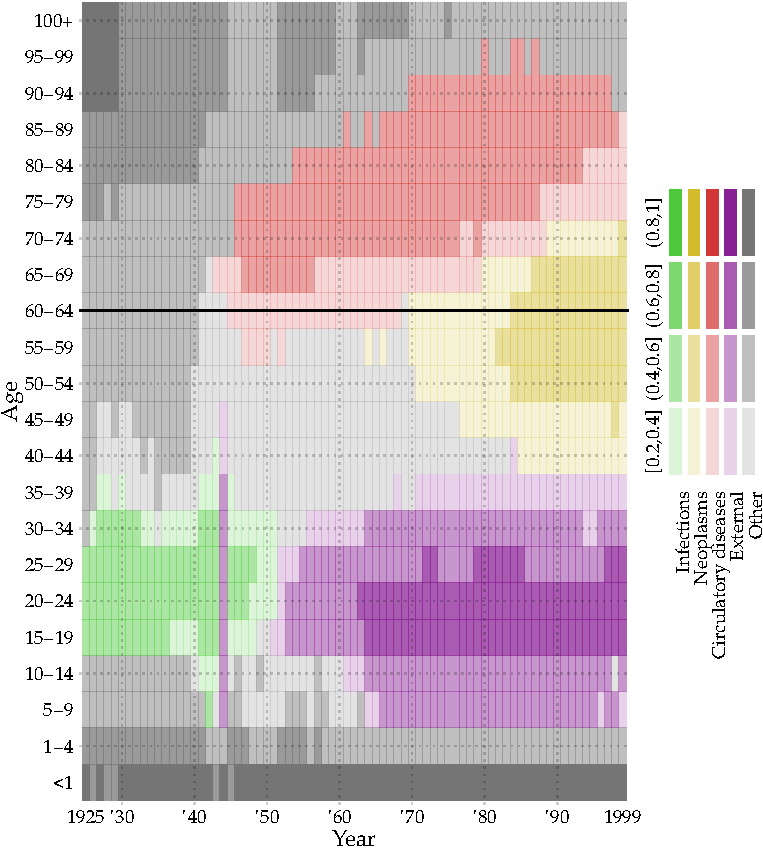
\includegraphics[width = 0.8\linewidth]{../fig/plot-qual_seq.pdf}
  \caption{Qualitative-sequential-scheme: Share of people dying from the most prominent cause in a given time and age (France, total population).}
  \label{fig:qss}
\end{figure}

One new insight this visualization yields is the importance of infectious diseases as a cause of death for people aged 15--40 prior to 1950. In these years and ages 20--60\,\% of the deceased die from infection making this the most likely cause of death in adolescence and middle-age. This pattern abruptly changes after 1950 with external causes of death taking the top spot. Similar to figure \ref{fig:tbs} we see the accident hump peaking around ages 15--30. Looking at data for five groups we get a more differentiated picture at the death causes in higher ages. Old age mortality is dominated by failures of the circulatory system. The onset of circulatory conditions as the main cause of death moves into higher ages in a linear fashion starting at around age 50 in the 1940s to age 70 in the 1990. For people with an extraordinarily long lifespan the death causes get more diverse with \enquote{other} causes of death in the lead.

While confined to visualize shares only for the most prominent group at any given point on the Lexis surface the qualitative-sequential scheme still reproduces a lot of the information gained from figure \ref{fig:tbs} while adding new insights. In cases where the changes of the group composition in the data are more subtle (no shift in order of group shares) this visualization would loose most of its explanatory power.

\section*{Age-wise-area-graph}

The \emph{stacked-area-chart} can be thought of as the continuous version of the stacked-bar-chart. Coloured areas indicate group shares which change along the x-axis. As the value of each individual group shares are indicated by \emph{length} as opposed to colour it is better suited to detect slight changes in group composition over time than the previous techniques. \textcite{Cleveland1984} show that people are able to decode visual information more precise into their numerical equivalents when it is represented by length and not by colour.

\begin{figure}[htb!]
  \centering
  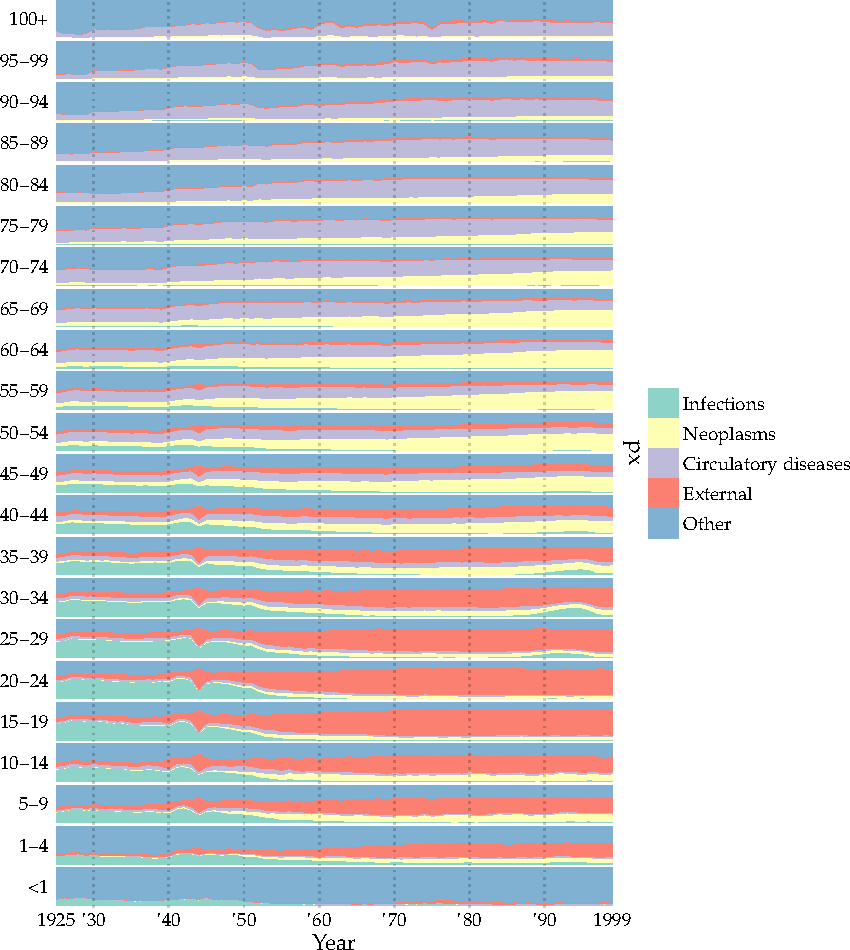
\includegraphics[width = 0.7\linewidth]{../fig/plot-agewise_area.pdf}
  \caption{Age-wise-area-graph: Proportion of people dying from a given cause by time and age (France, total population).}
  \label{fig:aag}
\end{figure}

For the \emph{age-wise}-area-graph we produce the stacked area chart separately for every age-group and assemble all of them on a Lexis-like grid. See figure \ref{fig:aag} for the resulting graph. Unlike with the ternary-balance-scheme we are able to distinguish more than three groups and unlike with the qualitative-sequential scheme the full information about the group distribution is retained.

One feature of the data which was hidden by the former graphical representations is the unusual surge in fatal infectious diseases in ages 25--40 around the mid 1990s. Looking at the exact cause of death data we see that HIV related deaths are a likely contributing factor to this local phenomena. Other new insights from this graph are the relative importance of cancer as a cause for childhood mortality and the high share of \enquote{other}-cause-mortality for people aged 90+.

The graph does not exhibit a true Lexis surface. The period-age grid is \emph{non-continuous} as it is composed of multiple stacked-area-charts each having a separate y-axis ranging from 0 (0\,\%) to 1 (100\,\%). This breaks the plot area into separate sections making the perception of global patterns harder because the global graphical patterns (the shape of the equal-colour areas across period and age) are interrupted along the age-scale. Also, while area charts (or continuous divided bar charts to stay within the vocabulary of Cleveland) are better than colour encodings for exact table-look up operations they are far from optimal for exact judgements about individual data values (\cite{Cleveland1994}).

The focus of the age-wise-area-graph lies on the detection of small local phenomena and developments within single age groups while still giving an overview of the global patterns for multiple groups on a single period-age-grid.

\section*{Small-multiples}

\emph{Small-multiples}\footnote{We use the terminology of \cite{Tufte1990}. Closely related concepts are \emph{facets} (\cite{Wilkinson2005}) or \emph{trellis-plots} (\cite{Becker1996}).} are related graphs displayed close to another differing only in the data dimension shown. They can be thought of as \enquote{tables of graphs} (\cite{Wilkinson2005}:319). Small-multiples are a fairly common technique and have already been discussed by \textcite{Vaupel1987} as a way of plotting mortality/fertility-surfaces for multiple sub-populations. We discuss this technique in the context of compositional data and propose a small adjustment facilitating cross-panel comparisons.

In figure \ref{fig:smg} we see multiple heatmaps of cause-specific shares of deaths in France across period and age. the graphs are augmented by border lines at calendar years and ages for which a given cause of death is dominant. Consider the first panel. It shows the proportion of deaths caused by infectious diseases by age and calendar time. Point \emph{A} indicates that in 1930 infectious diseases are the dominant cause of death for persons aged 30-34. Between 30--40\,\% of all deaths are caused by infection. Infectious diseases stop being the dominant cause of death around 1950. Injuries start to become dominant for persons between 1 and 40 in 1950. This leading position increases over time.

Unlike the other visualization techniques described in this paper the small-multiples allow us to display the death-shares for each of the 18 base-categories of ICD-9. This power of course comes with a price: The data is not contained in a single graphic. This means that the eye (and the mind) not only have to move between and compare different regions of a graph but make connections between different graphics in order to \emph{see the whole picture}. To make these comparisons easier we mark every period-age combination in which the corresponding cause of death has the highest share among all deaths with a black outline. This way it immediately becomes obvious where specific death causes dominate over all other death causes.

Again, the new visualization technique shines a different light on our data and allows for additional insights. We can see that ill-defined causes of death are common in the old ages. Also prior to World War II an ill-defined cause of death is the norm for people dying at ages 80 or higher. Perinatal conditions followed by congenital anomalies are the main causes of death for infants through most of the 20th century in France. Prior to 1950 deaths of infants and young children are, for the most part, attributed to respiratory diseases. For adults fatal respiratory diseases move into higher and higher ages, reaching a plateau around 1970 and being nearly exclusively an old-age phenomena from there on. A period-age effect can be identified in the realm of digestive diseases. The latter half of the 20th century sees a rise in the share of people aged 35-65 dying from conditions of the digestive system. However, note that the data is binned into 10\,\% categories simplifying a correct look-up of the colour values but forbidding the exact judgement of small differences.

\begin{landscape}

\begin{figure}[htb!]
  \centering
  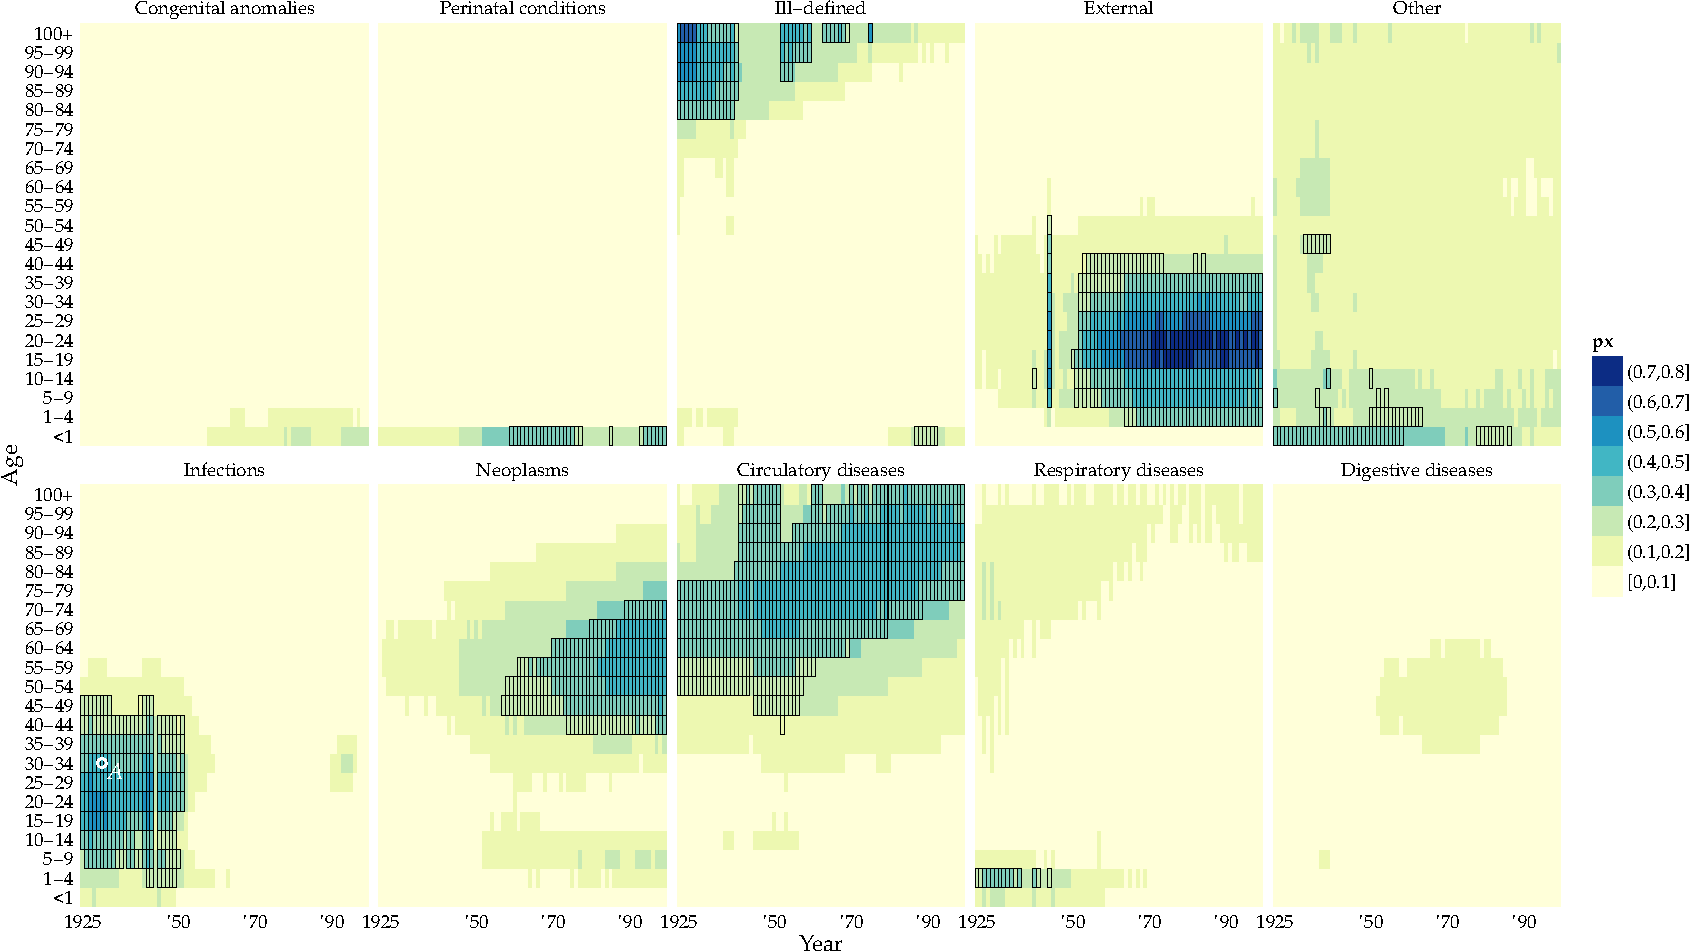
\includegraphics[width = \linewidth]{../fig/plot-small_multiples.pdf}
  \caption{Small-multiples: Proportion of people dying from a given cause by time and age (France, total population).}
  \label{fig:smg}
\end{figure}

\end{landscape}

\section*{Comparative evaluation}

If the visualization must contain \emph{complete} information about every group in the composition the qualitative-sequential-scheme is not an option as only the group with the highest share at a given period-age is considered. The remaining three techniques always show the complete distribution of group shares.

The Lexis surface approximates a \emph{continuous} grid of age by time. The age-wise-area graph breaks this essential feature by fracturing the surface into separate graphs by age. As each age group uses its own y-axis the surface becomes discontinuous along the age-axis. From a perceptional standpoint this hinders the identification of period- and cohort-effects as these would form continuous patterns along the age-(time)-axes but can not do so in the age-wise-area-graph. The remaining visualization techniques use a continuous Lexis surface.

The ternary-balance-scheme -- as the name suggests -- only allows for the display of ratios between three groups. If a visualization of proportions between a large \emph{number of groups} is required the small-multiples approach is best suited as a virtually unlimited number of group shares can be displayed at once.

The maximum number of groups allowed for in the qualitative-sequential-scheme and the age-wise-area-graphs is not restricted by principle but by perceptional limits. The qualitative-sequential scheme uses lightness steps within different hues to show different group shares. Therefore the number of groups which can sensibly be displayed at once is limited by the number of distinct hues one can perceive. Different lightness steps based on these hues should not be confused across hues. \textcite{Ware2013}:123 lists four unique hues: red, green, blue and yellow. These hues are are generally perceived as pure/unmixed colours which do not resemble each other. Yellow is problematic as a base hue for a lightness sequence as it is already a very light colour (\cite{Ware2013}:127). Orange, still being perceived distinct from red and yellow, is the better choice here. Adding black one can construct five sufficiently different lightness sequences. Some few additional hues, like purple, might also work.

The age-wise area-graphs contain a lot of information in a small vertical space. The more groups one adds the more crowded this vertical space gets and information retrieval will be more difficult.

The ternary-balance-scheme, the qualitative-sequential-scheme and the small-multiples are all heatmaps and differ only in the applied colour-scale. As such they are particularly suited to show patterns in the data such as period-, age- and cohort-effects or local outliers (as demonstrated for 1-dimensional data in \cite{Vaupel1987}). For the small-multiples approach this merit only applies to \emph{patter-perception} within groups as the information is spread out across multiple panels. The inter-group patterns are not directly visually encoded and have to be inferred from a comparison between multiple panels. The marking of modal values alleviates this task.

The case for age-wise-area-graphs is more complicated. Due to the discontinuities across the age dimension the global pattern-perception from these graphs is comparatively worse. However, changes over time within single age groups, even small ones, can be seen very well using this technique.\footnote{Given that no steep slopes occur or else there will be problems correctly judging the difference between the upper and lower boundary of an area -- the value (\cite{Cleveland1994}:227\,ff).}

None of the discussed techniques allows for a very efficient \emph{table look-up} operation (the quick and accurate retrieval of the underlying data values). Colour, as used by three out of the four techniques as encoding for the group shares, is generally regarded as the weakest graphical element in terms of table look-up (\cite{Cleveland1984}:536). The judgement of areas and lengths as used in the age-wise-area-graphs fares better, but the matter is complicated by the use of \emph{stacked-relative}-area-graphs. Here the value can only be directly read from the y-axis for the bottom group/area. For all other areas differences between two points on the y-axis equal the data value.

\emph{Space usage} of all techniques but the small-multiples is equal to a conventional heatmap across the same period-age-range. The small-multiples technique, depending on the number of groups, might be much larger up to the point of filling the whole page.

\begin{table}[!htb]
\tabformat
\begin{tabular}{p{3.5cm}*5{Q{1.5cm}}}
\toprule
 & Ternary-balance-scheme & Qualitative-sequential-scheme & Age-wise-area-graph & Small-multiples \\
\midrule
Sufficiency & yes & no & yes & yes \\
Continuity & yes & yes & no & yes \\
Category limit & 3 & $\approx$ 5--6 & $\approx 8$ & unlimited \\
Pattern perception & good & good & limited & good \\
Table look-up & limited & limited & limited & limited \\
Footprint & small & small & small & high \\
\bottomrule
\end{tabular}
\caption{Evaluation of different visualization techniques for compositional data on the Lexis surface}
\label{tab:eval}
\end{table}

\section*{Conclusion}

We demonstrated four different visualization techniques for showing cause of death distributions across period and age, extending the conventional period-age heatmap of 1-dimensional continuous data (e.g. surfaces of mortality rates) to multidimensional compositional data. We applied multivariate colour-scales originating from cartography to the Lexis surface (ternary-balance-scheme, qualitative-sequential-scheme), introduced age-wise area graphs as a means of visualizing compositional change over time within ages and improved upon the well known small multiple technique in the context of compositional data. Each of these techniques serves the cause of making sense of compositional data across time and age, while at the same time these techniques complement each other by having different strong points.

The ternary-balance-scheme is the best candidate for visualizing the \emph{shares of three groups}. Using principles of colour composition it produces smooth rainbow-like surfaces immediately indicating time-, age-, and cohort patterns in the data. The qualitative-sequential-scheme \emph{extends beyond three groups} and shows the shares of the most dominant groups on a surface. The age-wise-area-graphs use the power of the line to point out \emph{slight, age-specific changes} in group composition over time. Plotting a separate heatmap for each subgroup is a well-tried technique and still the most practical way to plot compositions for a \emph{large number of sub-groups}. Adding a contour line to each panel, indicating the regions of dominance of one group over the others, reduces the need for cross-panel comparisons and therefore adapts this proven technique further to the display compositional data.

What share of a population features attribute $i$ at period $t$ and age $x$? The proposed visualizations are tools helping to answer this question. We demonstrated the techniques using data on causes of death. Other possible applications include time-age surfaces of population shares by labour-market status (unemployed and seeking job, unemployed and not seeking job, employed), distributions of labour force over industries (agricultural, industry, service) or partnership status (single, in relationship and living alone, in relationship and cohabiting, married). The visualizations can also help interpreting the output from estimated models. The Heligman and Pollard model of overall life course mortality (\cite{Heligman1980}) for example is written as the sum of age-specific components for childhood-, accident- and senescent mortality. The relative magnitudes of these components can be clearly visualized using the ternary balance scheme, producing graphics of quasi cause-specific-mortality from all cause mortality data.

Good visualizations can be thought of as a visual model of the data at hand, able to identify relationships between variables. They go hand in hand with mathematical models of the data as both can be checked against the other. We hope to have contributed useful techniques for revealing information about compositions across time and age.

\clearpage

%%%% Bibliography %%%%%%%%%%%%%%%%%%%%%%%%%%%%%%%%%%%%%%%%%%%%%%%%%%%%%%%%%%%%%

\sloppy
\printbibliography

\clearpage

%%%% Appendix %%%%%%%%%%%%%%%%%%%%%%%%%%%%%%%%%%%%%%%%%%%%%%%%%%%%%%%%%%%%%%%%%

\begin{appendix}

\section{Construction of the ternary-balance-scheme}

There are multiple ways to construct the \emph{Ternary-balance-scheme}. To derive the scheme from a perceptual colour-space ensures that differences in the numeric data are mapped to perceptually equivalent differences in the colour representation. The perceived difference between any two hues should correspond to the difference between the underlying data values. Additionally a constant lightness of the colour-mixes is desirable as colour-lightness usually is assigned to the magnitude of a continuous variable (\cite{Brewer1994}), but we are dealing with compositional data which always sums up to the magnitude 1. The \emph{CIE-Lch} colour-space suits these needs as it is perceptually balanced and allows for the truly\footnote{Unlike the widely used HSV/HLS colour-spaces which confound the perceptual dimensions. Using these colour-spaces an increase in saturation also changes the perceived lightning of the colour (\cite{Brewer1999}).} independent specification of hue ($h$), chroma ($c$) and lightness ($L$) of a colour. The colour space can be thought of as a cylinder with different hues along the circumference, decreasing chroma along the radius towards the centre and increasing lightness along the vertical axis. Figure \ref{fig:cielch} shows a \enquote{slice} of this cylinder with a fixed lightness level. We will use this slice to construct the ternary-balance scheme for our graphic: In a first step the three groups in the data are assigned to \emph{equidistant} hues along the circumference of the circle. These are the base colours for each category. Next vectors originating from the centre and pointing towards the base colours are constructed. The length of each vector is given by the share of the corresponding group on the total. This share is then mapped to the available chroma range (in our example $[0,140]$, other upper limits are possible) with $c = 0$ corresponding to a share of 0\,\% and the upper limit of $c$ corresponding to 100\,\%. Finally the group specific vectors are added and the resulting vector returns the hue and chroma of the colour-mixture used to represent the distribution of the three groups. The possible colour-mixes form a triangular subset of the original CIE-Lch slice and therefore can be conveniently labelled with a ternary scale which allows for numerical interpretation of each mixed-colour (see figure \ref{fig:tern_construction}).

\begin{figure}[htb!]
  \begin{subfigure}[t]{0.3\textwidth}
  \centering
  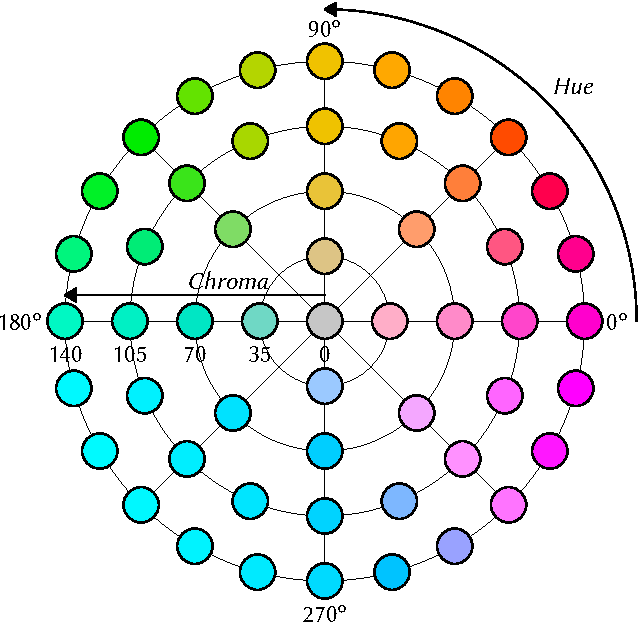
\includegraphics[width = \textwidth]{../fig/plot-cielch.pdf}
  \subcaption{CIE-Lch colour-space slice ($L = 80$).}
  \label{fig:cielch}
  \end{subfigure}%
  ~
  \begin{subfigure}[t]{0.3\textwidth}
  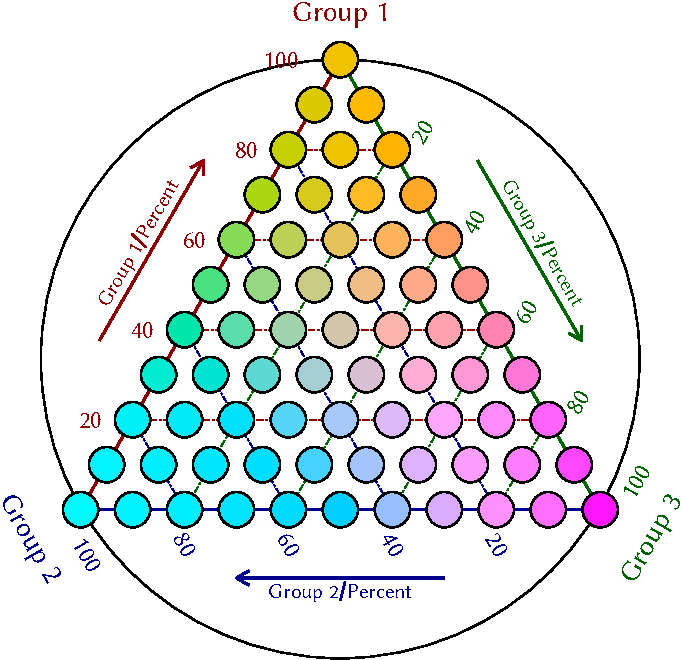
\includegraphics[width = \textwidth]{../fig/plot-ternary.pdf}
  \subcaption{Colour-mixes for different compositions of three groups derived from CIE-Lch.}
  \label{fig:ternlegend}
  \end{subfigure}%
  ~
  \begin{subfigure}[t]{0.3\textwidth}
  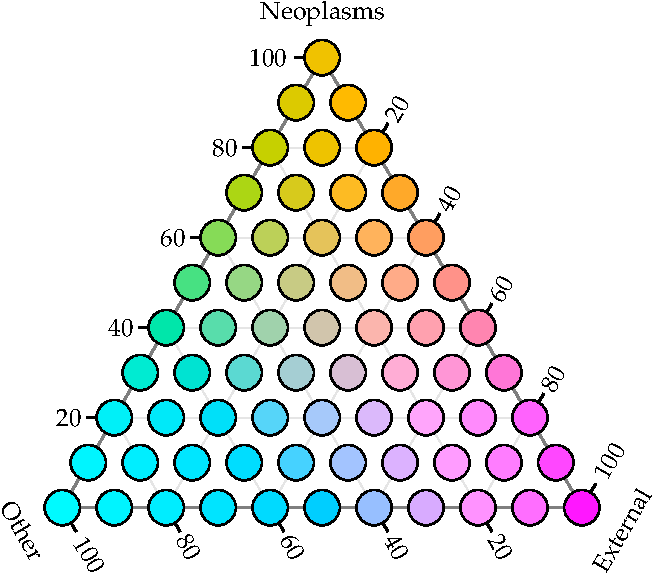
\includegraphics[width = \textwidth]{../fig/plot-tern_balance_lgnd.pdf}
  \subcaption{Legend for Ternary-balance-scheme graph of French cause of death proportions.}
  \label{fig:tbslegend}
  \end{subfigure}
  \caption{Con\-struc\-tion of the Ternary-balance-scheme.}
  \label{fig:tern_construction}
\end{figure}

\clearpage

\section{R code}

\lstinputlisting[caption=Initialization]{../R/01-init.R}
\clearpage
\lstinputlisting[caption=Utility Functions]{../R/02a-fnct_util.R}
\clearpage
\lstinputlisting[caption=Polar Coordinate Functions]{../R/02b-fnct_polar_coords.R}
\clearpage
\lstinputlisting[caption=Ternary Balance Scheme Functions]{../R/02c-fnct_ternary_balance.R}
\clearpage
\lstinputlisting[caption=Input]{../R/03-input.R}
\clearpage
\lstinputlisting[caption=Plot Ternary Balance Scheme]{../R/04a-plot_ternary_balance_scheme.R}
\clearpage
\lstinputlisting[caption=Plot Qualitative Sequential Scheme]{../R/04b-plot_qualitative_sequential_scheme.R}
\clearpage
\lstinputlisting[caption=Plot Age-Wise Area Chart]{../R/04c-plot_age-wise_area_chart.R}
\clearpage
\lstinputlisting[caption=Plot Small Multiples]{../R/04d-plot_small_multiples.R}

\end{appendix}

\end{document}